\documentclass[a4paper,11pt]{article}

\usepackage{mlsubmit}

\begin{document}

\initmlsubmision{1}                              					% assignment number
								{Nikhil Mittal}      						           		% your name
								{17111056}																		% your roll number

\begin{mlsolution}

Lerning with prototypes:\\
A two class problem where the prototypes are the points (1, 0) (green) and (0, 1) (red). Let the green point be \begin{math} \mu _{+} (1, 0) \end{math} and red point be \begin{math} \mu _{-} (0, 1) \end{math}. The decision boundary is the hyperplane where any point lying on the hyperplane is at equal distance from both the prototypes.
\\
1.  \begin{math}
 d\left ( z^{1}, \space z^{2} \right ) = \left \langle z^{1} - z^{2}, \space U\left ( z^{1} - z^{2} \right ) \right \rangle, U = \begin{bmatrix} 
3 & 0 \\ 0 & 1 \end{bmatrix} \\ 
\end{math}
\\
Let's take a point z \begin{math} \in \mathbb{R}^{2} \end{math}, finding it's distance from both the prototypes :
\\
So, z = \begin{math}
\begin{bmatrix} x\\ y \end{bmatrix},
\end{math} 
\begin{math}
\mu _{+} = \begin{bmatrix} 1\\ 0 \end{bmatrix} 
\end{math}
and
\begin{math}
\mu _{-} = \begin{bmatrix} 0\\ 1 \end{bmatrix}
\end{math}
\newline
\newline
\begin{math}
d\left ( \mu_{+}, \space z \right ) = \left \langle \mu_{+} - z, \space U\left ( \mu_{+} - z \right ) \right \rangle
\end{math}
\newline
\newline
\begin{math}
d\left ( \mu_{+}, \space z \right ) = \left \langle \begin{bmatrix} 1\\ 0 \end{bmatrix} - \begin{bmatrix} x\\ y \end{bmatrix} , \begin{bmatrix} 
3 & 0 \\ 0 & 1 \end{bmatrix} \left (  \begin{bmatrix} 1\\ 0 \end{bmatrix} - \begin{bmatrix} x\\ y \end{bmatrix}  \right ) \right \rangle
\end{math}
\newline
\begin{math}
d\left ( \mu_{+}, \space z \right ) = \left \langle \begin{bmatrix} 1-x\\ -y \end{bmatrix} , \begin{bmatrix} 
3 & 0 \\ 0 & 1 \end{bmatrix} \left (  \begin{bmatrix} 1-x\\ -y \end{bmatrix}  \right ) \right \rangle
\end{math}
\newline
\begin{math}
d\left ( \mu_{+}, \space z \right ) = \left \langle \begin{bmatrix} 1-x\\ -y \end{bmatrix} , \begin{bmatrix} 3*(1-x) \\ -y \end{bmatrix} \right \rangle
\\
\end{math}
\begin{math}
d\left ( \mu_{+}, \space z \right ) = \begin{bmatrix} 1-x\\ -y \end{bmatrix} ^{T}.\begin{bmatrix} 3*(1-x) \\ -y \end{bmatrix}\\ \\
d\left ( \mu_{+}, \space z \right ) = 3(1-x)^{2} + y^{2}
\end{math}
\newline
\begin{math}
\\
d\left ( \mu_{-}, \space z \right ) = \left \langle \mu_{-} - z, \space U\left ( \mu_{-} - z \right ) \right \rangle
\end{math}
\newline
\newline
\begin{math}
d\left ( \mu_{-}, \space z \right ) = \left \langle \begin{bmatrix} 0\\ 1 \end{bmatrix} - \begin{bmatrix} x\\ y \end{bmatrix} , \begin{bmatrix} 
3 & 0 \\ 0 & 1 \end{bmatrix} \left (  \begin{bmatrix} 0\\ 1 \end{bmatrix} - \begin{bmatrix} x\\ y \end{bmatrix}  \right ) \right \rangle
\end{math}
\newline
\begin{math}
d\left ( \mu_{-}, \space z \right ) = \left \langle \begin{bmatrix} -x\\ 1-y \end{bmatrix} , \begin{bmatrix} 
3 & 0 \\ 0 & 1 \end{bmatrix} \left (  \begin{bmatrix} -x\\1 -y \end{bmatrix}  \right ) \right \rangle
\end{math}
\newline
\begin{math}
d\left ( \mu_{-}, \space z \right ) = \left \langle \begin{bmatrix} -x\\ 1-y \end{bmatrix} , \begin{bmatrix} -3x \\ 1-y \end{bmatrix} \right \rangle
\end{math}
\newline
\begin{math}
\\
d\left ( \mu_{-}, \space z \right ) = \begin{bmatrix} -x\\ 1-y \end{bmatrix} ^{T}.\begin{bmatrix} -3x \\ 1-y \end{bmatrix}\\ \\
d\left ( \mu_{-}, \space z \right ) = 3x^{2} + (1-y)^{2}\\
\end{math}
Equate the difference of distances to decision boundary,\\
\begin{math}
f(z) = d\left ( \mu_{+}, \space z \right ) - d\left ( \mu_{-}, \space z \right )\\
\end{math}
For equation of f(z),
\begin{math}
f(z) = 0 \\
Then, d\left ( \mu_{+}, \space z \right ) - d\left ( \mu_{-}, \space z \right ) = 0\\
3(1-x)^{2} + y^{2} - 3x^{2} - (1-y)^{2} = 0\\
3(1 + x^{2} - 2
x) + y^{2} - 3x^{2} - (1 + y^{2} - 2y) = 0\
3 + 3x^{2} - 6x + y^{2} - 3x^{2} - 1 - y^{2} - 2y = 0\\
-6x + 2y + 2 = 0\\
y = 3x - 1
\end{math}\\\\
The mathematical expression for the decision boundary is :\\
 \begin{center}\boxed{ y = 3x - 1}\end{center}
    
\begin{figure}[th]%
\centering
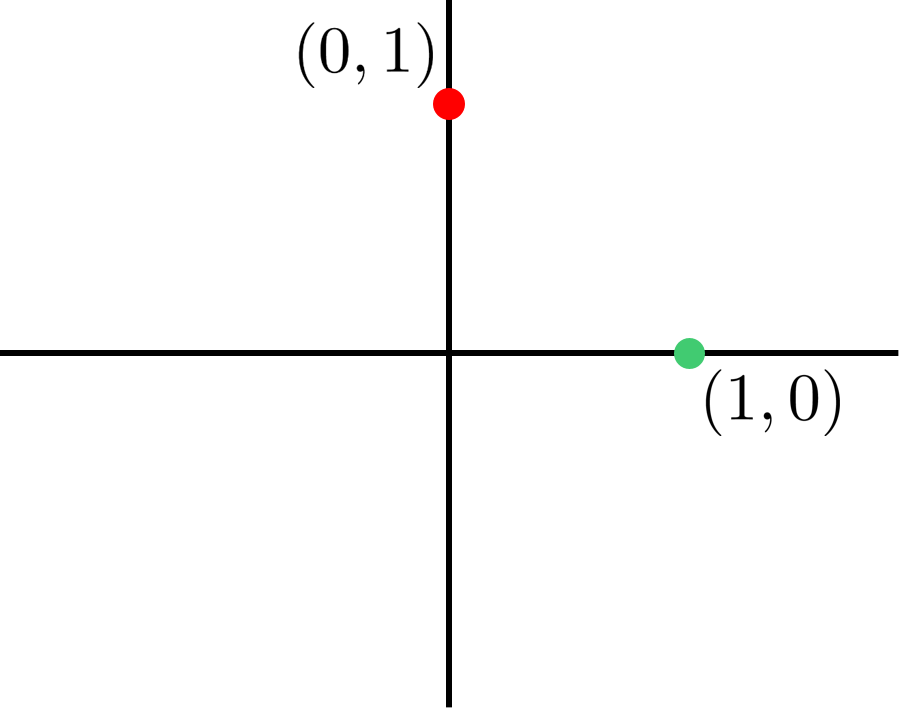
\includegraphics[width=0.3\columnwidth]{proto_blank.png}%
\hfill
\includegraphics[width=0.6\columnwidth]{Q1-1-1.png}%
\caption{Learning with Prototypes: the figure on the left shows the two prototypes. The figure on the right shows what the decision boundary if the distance measure used is $d(\vz^1,\vz^2) = \left \langle \vz^1-\vz^2, V (\vz^1-\vz^2) \right \rangle$, for any two points $\vz^1,\vz^2 \in \bR^2$. The decision boundary in this case is the line $y = 3x-1$.}%
\label{fig:proto1}%
\end{figure}

2.  \begin{math}
 d\left ( z^{1}, \space z^{2} \right ) = \left \langle z^{1} - z^{2}, \space V \left ( z^{1} - z^{2} \right ) \right \rangle, V = \begin{bmatrix} 
1 & 0 \\ 0 & 0 \end{bmatrix} \\ \end{math}

Let's take a point z \begin{math} \in \mathbb{R}^{2} \end{math}, finding it's distance from both the prototypes :
\\
So, z = \begin{math}
\begin{bmatrix} x\\ y \end{bmatrix},
\end{math} 
\begin{math}
\mu _{+} = \begin{bmatrix} 1\\ 0 \end{bmatrix} 
\end{math}
and
\begin{math}
\mu _{-} = \begin{bmatrix} 0\\ 1 \end{bmatrix}
\end{math}
\newline
\newline
\begin{math}
d\left ( \mu_{+}, \space z \right ) = \left \langle \mu_{+} - z, \space V\left ( \mu_{+} - z \right ) \right \rangle
\end{math}
\newline
\newline
\begin{math}
d\left ( \mu_{+}, \space z \right ) = \left \langle \begin{bmatrix} 1\\ 0 \end{bmatrix} - \begin{bmatrix} x\\ y \end{bmatrix} , \begin{bmatrix} 
1 & 0 \\ 0 & 0 \end{bmatrix} \left (  \begin{bmatrix} 1\\ 0 \end{bmatrix} - \begin{bmatrix} x\\ y \end{bmatrix}  \right ) \right \rangle
\end{math}
\newline
\begin{math}
d\left ( \mu_{+}, \space z \right ) = \left \langle \begin{bmatrix} 1-x\\ -y \end{bmatrix} , \begin{bmatrix} 
1 & 0 \\ 0 & 0 \end{bmatrix} \left (  \begin{bmatrix} 1-x\\ -y \end{bmatrix}  \right ) \right \rangle
\end{math}
\newline
\begin{math}
d\left ( \mu_{+}, \space z \right ) = \left \langle \begin{bmatrix} 1-x\\ -y \end{bmatrix} , \begin{bmatrix} 1-x \\ 0 \end{bmatrix} \right \rangle
\\
\end{math}
\begin{math}
d\left ( \mu_{+}, \space z \right ) = \begin{bmatrix} 1-x\\ -y \end{bmatrix} ^{T}.\begin{bmatrix} 1-x \\ -y \end{bmatrix}\\ \\
d\left ( \mu_{+}, \space z \right ) = (1-x)^{2}
\end{math}
\newline
\begin{math}
\\
d\left ( \mu_{-}, \space z \right ) = \left \langle \mu_{-} - z, \space V\left ( \mu_{-} - z \right ) \right \rangle
\end{math}
\newline
\newline
\begin{math}
d\left ( \mu_{-}, \space z \right ) = \left \langle \begin{bmatrix} 0\\ 1 \end{bmatrix} - \begin{bmatrix} x\\ y \end{bmatrix} , \begin{bmatrix} 
1 & 0 \\ 0 & 0 \end{bmatrix} \left (  \begin{bmatrix} 0\\ 1 \end{bmatrix} - \begin{bmatrix} x\\ y \end{bmatrix}  \right ) \right \rangle
\end{math}
\newline
\begin{math}
d\left ( \mu_{-}, \space z \right ) = \left \langle \begin{bmatrix} -x\\ 1-y \end{bmatrix} , \begin{bmatrix} 
1 & 0 \\ 0 & 0 \end{bmatrix} \left (  \begin{bmatrix} -x\\1 -y \end{bmatrix}  \right ) \right \rangle
\end{math}
\newline
\begin{math}
d\left ( \mu_{-}, \space z \right ) = \left \langle \begin{bmatrix} -x\\ 1-y \end{bmatrix} , \begin{bmatrix} -x \\ 0 \end{bmatrix} \right \rangle
\end{math}
\newline
\begin{math}
\\
d\left ( \mu_{-}, \space z \right ) = \begin{bmatrix} -x\\ 1-y \end{bmatrix} ^{T}.\begin{bmatrix} -x \\ 0 \end{bmatrix}\\ \\
d\left ( \mu_{-}, \space z \right ) = x^{2} \\
\end{math}
Equate the difference of distances to decision boundary,\\
\begin{math}
f(z) = d\left ( \mu_{+}, \space z \right ) - d\left ( \mu_{-}, \space z \right )\\
\end{math}
For equation of f(z),
\begin{math}
f(z) = 0 \\
Then, d\left ( \mu_{+}, \space z \right ) - d\left ( \mu_{-}, \space z \right ) = 0\\
(1-x)^{2} - x^{2} = 0\\
1 + x^{2} - 2x - x^{2} = 0\\
1 - 2x = 0\\
x = \frac{1}{2} \\
\end{math}\\
The mathematical expression for the decision boundary is :\\
\begin{center} \begin{math} \boxed{x = \frac{1}{2}} \end{math} \end{center}

\begin{figure}[th]%
\centering
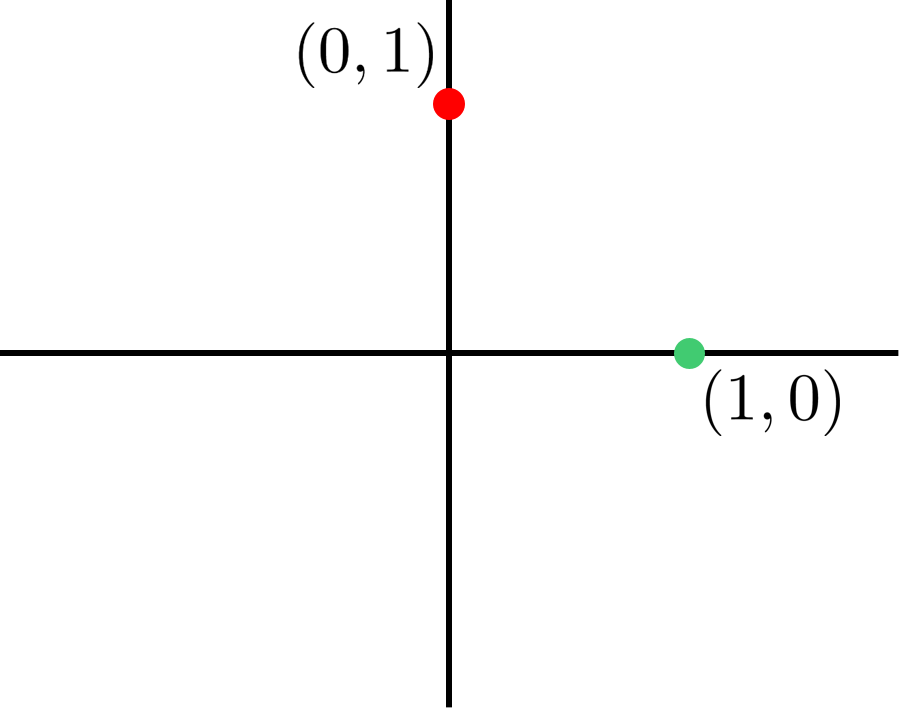
\includegraphics[width=0.3\columnwidth]{proto_blank.png}%
\hfill
\includegraphics[width=0.7\columnwidth]{Q1-2-1.png}%
\caption{Learning with Protypes: the figure on the left shows the two prototypes. The figure on the right shows what the decision boundary if the distance measure used is $d(\vz^1,\vz^2) =\left \langle \vz^1-\vz^2, U (\vz^1-\vz^2) \right \rangle$, for any two points $\vz^1,\vz^2 \in \bR^2$. The decision boundary in this case is the line $x = 1/2$.}%
\label{fig:proto2}%
\end{figure}

\end{mlsolution}

\begin{mlsolution}
Second answer

\end{mlsolution}

\begin{mlsolution}
We need to design a likelihood and prior distribution such that $\hat\vw_\text{fr}$ this is the map estimate.
\\The Posterior distribution on \textbf{w} can be seen as proportional to the product of the likelihood and the prior distributions.

Let's take the gaussian likelihood and gaussian prior,
\\Here \textbf
X
 is \textbf{n}*\textbf{d} matrix where \textbf{n} is the no. of data points and \textbf{d} is the no. of features.
\\\\
\[
P[y^{i}|x^{i}, w] = \mathcal{N} \left ( \left \langle w, x^{i} \right \rangle, \sigma^{2} \right ) 
\\
= \frac{1}{{\sigma \sqrt {2\pi } }}e^{{{ - \left( {y^{i} - \left \langle w, x^{i} \right \rangle } \right)^2 } \mathord{\left/ {\vphantom {{ - \left( {y^{i} - \left \langle w, x^{i} \right \rangle } \right)^2 } {2\sigma ^2 }}} \right. \kern-\nulldelimiterspace} {2\sigma ^2 }}}
\]\\

\[
\text{P}[\textbf{y} | \textbf{X}, \textbf{w}] = 
= \frac{1}{{\sigma \sqrt {2\pi } }} \prod_{i=1}^{n} e^{{{ - \left( {y^{i} - \left \langle w, x^{i} \right \rangle } \right)^2 } \mathord{\left/ {\vphantom {{ - \left( {y^{i} - \left \langle w, x^{i} \right \rangle } \right)^2 } {2\sigma ^2 }}} \right. \kern-\nulldelimiterspace} {2\sigma ^2 }}}

\]
So Log likelihood will be :
\\\\
\begin{math}
\log P[\textbf{y} | \textbf{X}, \textbf{w}] = C - \frac{1}{2\sigma^{2}} \sum_{i = 1}^{n} \left ( y^{i} - \left \langle \textbf{w}, \textbf{x}^{i} \right \rangle \right )^{2}
\end{math}
\\\\Taking Gaussian prior, with a minor modification :\\\\Consider a \begin{math} \beta \end{math} Such that \[ \beta = \left [ \frac{1}{\beta_{1}}\;\; \frac{1}{\beta_{2}}\;\; .\;..  \;\;\frac{1}{\beta_{d}} \right ] , \beta_{j} > 0\] and d is the dimension of \beta.\\Then, \[ \text{I}{}' = \beta\cdot\vI\] Where $\vI$ is the identity matrix.\\

\[ \text{I}{}' = \begin{bmatrix}
\frac{1}{\beta_{1}} & 0 & . & . & 0\\ 
0 & \frac{1}{\beta_{2}} & . & . & 0 \\ 
0 & . & . & . & 0\\ 
0 & . & . & . & 0\\ 
0 & . & . & . & \frac{1}{\beta_{d}}
\end{bmatrix}\]

Using Gaussian prior, 
\[
P[\textbf{w}] = \mathcal{N}\left ( 0, \rho^{2}.\text{I}{}' \right ) = \frac{1}{\sqrt{\left ( 2\pi \right)^{d}\rho^{2}\left | \text{I}{}' \right |}}\exp\left ( - \frac{\textbf{w}^T\text{I}{}'^{-1}\textbf{w}}{2\rho^{2}} \right )
\]

Actually \text{I}{}' is diagonal matrix. So, It's inverse is :

\[
    \text{I}{}'^{-1} = \begin{bmatrix}
\beta_{1} & 0 & . & . & 0\\ 
0 & \beta_{2} & . & . & 0 \\ 
0 & . & . & . & 0\\ 
0 & . & . & . & 0\\ 
0 & . & . & . & \beta_{d}
\end{bmatrix}
\]

So, 
\[
\textbf{w}^T\text{I}{}'^{-1}\textbf{w} = \sum_{i=1}^{d}   \beta_j \left ( \textbf{w}_{j} \right )^{2}
\]
So, 
\begin{math}
P[\textbf{w}] = \mathcal{N}\left ( 0, \rho^{2}.I_{d} \right ) = \frac{1}{\sqrt{\left ( 2\pi \right)^{d}\rho^{2}}}\exp\left ( - \frac{\sum_{j = 1}^{d} \beta_{j}\left ( \textbf{w}_{j} \right )^{2} }{2\rho^{2}} \right )
\end{math}
\\Taking log we get :\\

\begin{math}
\log \end{math}\;P\begin{math}[\textbf{w}]  = C^{'} - \frac{1}{2\rho^{2}} \sum_{j = 1}^{d} \beta_{j}\left ( \textbf{w}_{j} \right )^{2} 
\end{math}\\\\So the posterior distribution on \textbf{w} :\\

P \begin{math}[\textbf{w}\mid\textbf{X},\textbf{y}]  \propto \end{math}\;P\begin{math}[\textbf{y}|\textbf{X}, \textbf{w}] . \end{math}\;P\begin{math}[\textbf{w}]\end{math}\\

\begin{math}
\log P[\textbf{w}\mid\textbf{X},\textbf{y}]  = \log P[\textbf{y}|\textbf{X}, \textbf{w}] + \log P[\textbf{w}]
\end{math}\\

\begin{math}
\widehat{\textbf{w}}_{\textbf{MAP}}  = \arg \underset{\textbf{w}}{\max} \log P[\textbf{y}|\textbf{X}, \textbf{w}] + \log P[\textbf{w}]
\end{math}\\
Using the expressions of log-likelihood and log-prior, we can say that :\\

\begin{math}
\widehat{\textbf{w}}_{\textbf{MAP}}  = \arg \underset{\textbf{w}}{\max} \;
C - \frac{1}{2\sigma^{2}} \sum_{i = 1}^{n} \left ( y^{i} - \left \langle \textbf{w}, \textbf{x}^{i} \right \rangle \right )^{2} + C^{'} - \frac{1}{2\rho^{2}} \sum_{j = 1}^{d} \beta_{j}\left ( \textbf{w}_{j} \right )^{2}
\end{math}\\\\
Ignoring constants \\

\begin{math}
\widehat{\textbf{w}}_{\textbf{MAP}}  = \arg \underset{\textbf{w}}{\min} \;
\frac{1}{2\sigma^{2}} \sum_{i = 1}^{n} \left ( y^{i} - \left \langle \textbf{w}, \textbf{x}^{i} \right \rangle \right )^{2} + \frac{1}{2\rho^{2}} \sum_{j = 1}^{d} \beta_{j}\left ( \textbf{w}_{j} \right )^{2}
\end{math}\\\\
Multiplying the equation by \begin{math}2\sigma^{2}\end{math}, we get Equation 1:\\

\begin{math}
\widehat{\textbf{w}}_{\textbf{MAP}}  = \arg \underset{\textbf{w}}{\min} \; \sum_{i = 1}^{n} \left ( y^{i} - \left \langle \textbf{w}, \textbf{x}^{i} \right \rangle \right )^{2} + \frac{\sigma^{2}}{\rho^{2}} \sum_{j = 1}^{d} \beta_{j}\left ( \textbf{w}_{j} \right )^{2}
\end{math}\\\\
Let's take \begin{math}\alpha_{j}\end{math} , such that \begin{math} \alpha_{j} = \frac{\sigma^{2}}{\rho^{2}}.\beta_{j}  \end{math}.
Such that \begin{math} \alpha = \left \{ \alpha_{1}, \alpha_{2}, ..., \alpha_{d} \right \} , \alpha_{j} > 0\end{math}  and d is the dimension.
So Equation 1 changes to :\\

\begin{math}
\widehat{\textbf{w}}_{\textbf{MAP}}  = \arg \underset{\textbf{w}}{\min} \; \sum_{i = 1}^{n} \left ( y^{i} - \left \langle \textbf{w}, \textbf{x}^{i} \right \rangle \right )^{2} + \sum_{j = 1}^{d} \alpha_{j}\left ( \textbf{w}_{j} \right )^{2}
\end{math}\\\\This is similar to the \begin{math}\widehat{\textbf{w}}_{fr}\end{math} as given in the question.\\It has a closed form solution which can be derived as follows : \\\\Take derivative of \begin{math}\widehat{\textbf{w}}_{fr}\end{math} w.r.t \textbf{w}\\\\

\begin{math}
\frac{ d\widehat{\textbf{w}}_{\textbf{fr}} }{dx} = \left ( 2 \right ) \sum_{i = 1}^{n}\left ( y^{i} - \left \langle \textbf{w}, \textbf{x}^{i} \right \rangle \right )\left ( - \textbf{x}^{i} \right ) + \frac{d}{dw} (\sum_{j = 1}^{d} \alpha_{j}\left ( \textbf{w}_{j} \right )^{2})
\end{math}\\

\begin{math}
\frac{ d\widehat{\textbf{w}}_{\textbf{fr}} }{dx} = \left ( -2 \right ) \sum_{i = 1}^{n}\left ( \textbf{x}^{i}y^{i} - \textbf{x}^{i}\left \langle \textbf{w}, \textbf{x}^{i} \right \rangle \right  ) + \sum_{j = 1}^{d} \frac{d}{d\textbf{w}_{j}} (\alpha_{j}\left ( \textbf{w}_{j} \right )^{2})
\end{math}\\

\begin{math}
\frac{ d\widehat{\textbf{w}}_{\textbf{fr}} }{dx} = \left ( -2 \right ) \sum_{i = 1}^{n}\left ( \textbf{x}^{i}y^{i} - \textbf{w}. (\textbf{x}^{i})^{2} \right  ) + \sum_{j = 1}^{d} (2\alpha_{j}\textbf{w}_{j})
\end{math}\\

\begin{math}
\frac{ d\widehat{\textbf{w}}_{\textbf{fr}} }{dx} = \left ( -2 \right ) \sum_{i = 1}^{n}\left ( \textbf{x}^{i}y^{i} \right  )  + 2 \; \textbf{w}.\sum_{i=1}^{n} (\textbf{x}^{i})^{2} + 2 \alpha^{T}\textbf{w}
\end{math}\\\\ Equating this equation to zero to get the value of \textbf{w}, We get :\\

\begin{math}
\textbf{w}.\sum_{i=1}^{n} (\textbf{x}^{i})^{2} + \alpha^{T}\textbf{w} = \sum_{i = 1}^{n}\left ( \textbf{x}^{i}y^{i} \right  ) 
\end{math}\\

\begin{math}
\textbf{w}\textbf{X}^{T}\textbf{X} + \alpha^{T}\textbf{w} = \textbf{X}^{T}\textbf{Y}
\end{math}\\

\begin{math}
\textbf{w}\left ( \textbf{X}^{T}\textbf{X} + \alpha^{T}I \right ) = \textbf{X}^{T}\textbf{Y}\end{math}\\

\begin{math}
\textbf{w} = \left ( \textbf{X}^{T}\textbf{X} + \alpha^{T}I \right )^{-1} \textbf{X}^{T}\textbf{Y}
\end{math}\\
\\So this is the closed form expression for \begin{math}\widehat{\textbf{w}}_{fr}\end{math} :

\begin{math}
\widehat{\textbf{w}}_{fr} = \left ( \textbf{X}^{T}\textbf{X} + \alpha^{T}I \right )^{-1} \textbf{X}^{T}\textbf{Y}
\end{math}\\

\end{mlsolution}

\begin{mlsolution}

\begin{math}
\left \{ \widehat{\textbf{W}}, \left \{ \widehat{\xi _{i}} \right \} \right \} = \underset{\textbf{W},}{arg} \; \underset{ \left \{ \widehat{\xi _{i}} \right \}}{min} \sum_{k=1}^{K} \left \| \textbf{w}^{k} \right \|^{2}_{2} + \sum_{i=1}^{n} \xi _{i}\end{math}\\\\

\begin{math}
\;\;\;\;s.t. \left \langle \textbf{w}^{y^{i}}, x^{i} \right \rangle \geq \left \langle \textbf{w}^{k}, x^{i} \right \rangle + 1 - \xi_{i}\; , \forall i\; \forall k\neq y^{i} \\
\end{math}\\

\begin{math}
\; \; \; \; \xi_{i} \geq 0, \forall i
\end{math}
So \begin{math}\widehat{\xi _{i}}\end{math} is for every data point.\\

The given constraint: \; \; \begin{math} \left \langle \textbf{w}^{y^{i}}, x^{i} \right \rangle \geq \left \langle \textbf{w}^{k}, x^{i} \right \rangle + 1 - \xi_{i}\; , \forall i\; \forall k\neq y^{i} \\ \end{math} \\

\begin{math} \xi_{i} \geq \left \langle \textbf{w}^{k}, x^{i} \right \rangle + 1 - \left \langle \textbf{w}^{y^{i}}, x^{i} \right \rangle \; , \forall i\; \forall k\neq y^{i} \\ \end{math} \\

\begin{math}
\xi_{i} \geq 1 + \left \langle \textbf{w}^{k}, x^{i} \right \rangle - \left \langle \textbf{w}^{y^{i}}, x^{i} \right \rangle \; , \forall i\; \forall k\neq y^{i} \\
\end{math}

So we can safely say that :
\begin{math}
\xi_{i} = \max\left (   1 + \left \langle \textbf{w}^{k}, x^{i} \right \rangle - \left \langle \textbf{w}^{y^{i}}, x^{i} \right \rangle \; \right ), \forall i,\; \forall k\neq y^{i} \\
\end{math}

As,\begin{math} \eta ^{i} = \left \langle \textbf{W}, \textbf{x}^{i} \right \rangle \Rightarrow \eta_{k} ^{i} = \left \langle \textbf{w}^{k}, \textbf{x}^{i} \right \rangle  and \;\eta_{y} ^{i} = \left \langle \textbf{w}^{y^{i}}, \textbf{x}^{i} \right \rangle \end{math}\\

\begin{math}
\xi_{i} \geq 1 + \eta_{k}^{i} - \eta_{y} ^{i} \;\;\; \forall k\neq y^{i} \\
\end{math}

\begin{math}
\xi_{i}
\end{math} is evaluated for all \begin{math}\textbf{w} \in \textbf{W}\end{math}, except for k \begin{math}\neq\end{math} y. We will take the largest possible value for \begin{math}\xi_{i}\end{math}. So \begin{math}\xi_{i}\end{math} will be maximum only when \begin{math}\eta_{k}\end{math} is maximum, satisfying the condition that \begin{math}k \neq y\end{math}.\\

So \begin{math}\xi_{i}\end{math} can be s.t., \begin{math}
\xi_{i} \geq 1 + \max \eta_{k}^{i} - \eta_{y} ^{i} \;\;\; \forall k\neq y^{i} \\
\end{math}, but because of the objective we will not want to set it any larger than necessary. As setting larger than that value will be unnecessary in the objective.\\

\begin{math}\xi_{i} =   1 + \underset{k\neq y}{\max} \;\eta_{k}^{i} - \eta_{y} ^{i}  \end{math}\;and\;\begin{math} \xi_{i}\geq 0\end{math}

Therefore \begin{math} \xi_{i}\end{math} is always a positive function and can be written as :

\begin{math}\xi_{i} =   \left [  1 + \underset{k\neq y}{\max} \;\eta_{k}^{i} - \eta_{y} ^{i}\;\right ]_{+}\end{math}

The above is same as \begin{math} l_{cs}\left ( y^{i},\eta ^{i} \right ) \end{math}.\\ It is called as the crammer-singer loss function.

Hence, \begin{math} l_{cs}\left ( y^{i},\eta ^{i} \right ) = \xi _{i} \end{math}\\

So the constrained formulation can now be written in an unconstrained formulation which is same as (P2). As \begin{math} \xi _{i} \end{math} can be replaced by \begin{math} l_{cs}\end{math}. Hence by this expression (P2) can be derived from (P1) and vice-versa.

Suppose \begin{math} \left \{ \textbf{W}^{0}, \left \{ \xi _{i}^{0} \right \} \right \} \end{math} is the optimum for P1 equation.

So \begin{math}\xi_{i}\end{math} satisfies the cosntraints.\\

For \begin{math} \left \{ \textbf{W}^{0}, \left \{ \xi _{i}^{0} \right \} \right \} \end{math} the sum \begin{math}  \end{math} is minimum. Such that 

\begin{math}\xi_{i}^{0} =  \max \left ( 1 + \left \langle \textbf{w}^{k}, x^{i} \right \rangle - \left \langle \textbf{w}^{y^{i}}, x^{i} \right \rangle\right )  \;and\; \xi_{i}\geq 0
\end{math}\\

So, 
\begin{math}\xi_{i}^{0} =   1 + \underset{k\neq y}{\max} \;\eta_{k}^{i} - \eta_{y} ^{i}  \;and\; \xi_{i}\geq 0\end{math}

Since \begin{math}\xi_{i}^{0} \geq 0\end{math}  \;so \; \begin{math} 1 + \underset{k\neq y}{\max} \;\eta_{k}^{i} - \eta_{y} ^{i} \geq 0 \end{math}

As stated \begin{math} l_{cs}\left ( y^{i},\eta ^{i} \right ) \end{math}.\\ 

Hence \begin{math} l_{cs} = \xi_{i}^{0}\end{math}, So the problem (P2) after plugging the value of \begin{math} l_{cs} \end{math} becomes similar to (P1).\\

(P2) is :\\

\begin{math}\left \{ \widehat{\textbf{W}} \right \} = \underset{\textbf{}}{arg} \; \underset{  \textbf{W}}{min} \sum_{k=1}^{K} \left \| \textbf{w}^{k} \right \|^{2}_{2} + \sum_{i=1}^{n} l _{cs}\left ( y^{i}, \eta ^{i} \right )\end{math}\\

Then, Put value of \begin{math} l_{cs}\end{math}. The problem becomes,\\

\begin{math}\left \{ \widehat{\textbf{W}} \right \} = \underset{\textbf{}}{arg} \; \underset{  \textbf{W}}{min} \sum_{k=1}^{K} \left \| \textbf{w}^{k} \right \|^{2}_{2} + \sum_{i=1}^{n} \xi_{i}^{0}\end{math}\\

As we know that above has minimum at \begin{math}\left \{ \textbf{W}^{0}, \left \{ \xi _{i}^{0} \right \} \right \} \end{math}

This problem is already solved as we know, \begin{math}\textbf{W}^{0}\end{math} minimizes  \begin{math}\sum_{k=1}^{K} \left \| \textbf{w}^{k} \right \|^{2}_{2}\end{math} and the \begin{math}\sum_{i=1}^{n} \xi_{i}^{0}\end{math} is just a constant and is already the optimal value.\\

So \begin{math}\textbf{W}^{0}\end{math} is also a solution for (P2).\\

Now, \begin{math}\textbf{W}^{1}\end{math} is an optimum for (P2). This means :\\

\begin{math}\left \{ \widehat{\textbf{W}} \right \} = \underset{\textbf{}}{arg} \; \underset{  \textbf{W}}{min} \sum_{k=1}^{K} \left \| \textbf{w}^{k} \right \|^{2}_{2} + \sum_{i=1}^{n} l _{cs}\left ( y^{i}, \eta ^{i} \right )\end{math} has minima at \begin{math}\textbf{W}^{1}\end{math}.\\

\begin{math}
\sum_{i=1}^{n} l_{cs} (y^{i}, \eta^{i}) 
\end{math} is the sum of losses, it is same for every \textbf{i}.\\

\begin{math}l_{cs}(y^{i}, \eta^{i}) =   \left [  1 + \underset{k\neq y}{\max} \;\eta_{k}^{i} - \eta_{y} ^{i}\;\right ]_{+}\end{math}\\

\begin{math}
\eta_{k} ^{i} = \left \langle \textbf{w}^{k}, \textbf{x}^{i} \right \rangle  and \;\eta_{y} ^{i} = \left \langle \textbf{w}^{y^{i}}, \textbf{x}^{i} \right \rangle
\end{math}\\

\begin{math}l_{cs}(y^{i}, \eta^{i}) \geq \left [  1 +  \;\left \langle \textbf{w}^{k}, \textbf{x}^{i} \right \rangle - \left \langle \textbf{w}^{y^{i}}, \textbf{x}^{i} \right \rangle\;\right ]_{+}\forall i; \;\forall k \neq y^{i}\end{math}. 
As \begin{math}l_{cs}(y^{i}, \eta^{i})\end{math} is the maximum value so this inequality should be satisfied. \\
As \begin{math}l_{cs}(y^{i}, \eta^{i})\end{math} is the maximum value so this inequality should be satisfied. \\

So we can say that there is some \begin{math}
\xi_{i}^{1}\end{math} which is equivalent to \begin{math}l_{cs}(y^{i}, \eta^{i})\end{math} and \begin{math} \xi_{i}^{1} \geq 0 \end{math} as \begin{math}l_{cs}(y^{i}, \eta^{i}) \geq 0 \end{math}.\\

Therefore, 
\begin{math} \xi_{i}^{1}  \geq  1 +  \;\left \langle \textbf{w}^{k}, \textbf{x}^{i} \right \rangle - \left \langle \textbf{w}^{y^{i}}, \textbf{x}^{i} \right \rangle\;\forall i; \;\forall k \neq y^{i}\end{math} \\

So the \begin{math}
\sum_{i=1}^{n} \xi_{i}^{1} 
\end{math} is minimum as it is same as \begin{math}\sum_{i=1}^{n} l_{cs}\end{math}.\\

So If I plug in \begin{math} \xi_{i} \end{math} in (P2) instead of \begin{math}
l_{cs}\end{math}. So it becomes constrained problem instead of unconstrained, but the meaning remains same.\\

So, \begin{math}
\sum_{k=1}^{K} \left \| \textbf{w}^{k} \right \|^{2}_{2} + \sum_{i=1}^{n} \xi _{i}
\end{math} has  \begin{math}
\min
\end{math} at \begin{math}\textbf{W}^{1} \end{math} and \begin{math}
\left \{\xi_{i}\right \}\end{math} value as \begin{math}\left \{ \xi_{i}^{1}\right \} \end{math}, as it is optimum.\\\\

\begin{math}
\left \{ \widehat{\textbf{W}}, \left \{ \widehat{\xi _{i}} \right \} \right \} = \underset{\textbf{W},}{arg} \; \underset{ \left \{ \widehat{\xi _{i}} \right \}}{min} \sum_{k=1}^{K} \left \| \textbf{w}^{k} \right \|^{2}_{2} + \sum_{i=1}^{n} \xi _{i}\end{math}  \;has optimum at \begin{math} \left \{ \textbf{W}^{1}, \left \{ \xi _{i}^{1} \right \} \right \} \end{math}.\\\\

Therefore (P1) and (P2) are equivalent.

\end{mlsolution}

\begin{mlsolution}

\begin{math}f \left ( \textbf{w} \right ) = \sum_{i=1}^{n} \left [  1 - y^{i}<\textbf{w}, x^{i}> \right ]_{+}\end{math}\\

\begin{math}
= \sum_{i=1}^{n} \textbf{v}\left ( x^{i}, y^{i} \right ),\end{math} such that \begin{math}\textbf{v}\left ( x^{i}, y^{i} \right ) = \left\{\begin{matrix}
1 - y^{i}<\textbf{w}, x^{i}> &, y^{i}<\textbf{w}, x^{i}> \;<  1\\
0 & , y^{i}<\textbf{w}, x^{i}> \;\geq  1
\end{matrix}\right.
\end{math}

\begin{math}
f\left ( \textbf{w} \right )
\end{math} is just the sum of hinge losses, where hinge function is not differentiable at \begin{math}y^{i}<\textbf{w}, x^{i}> = 1\end{math} . To find the sub-differential of f at w, \\

\begin{math}
\frac{df\left ( \textbf{w} \right )}{d\textbf{w}} = \sum \frac{dv\left ( x^{i}, y^{i} \right )}{d\textbf{w}}
\end{math}\\

\begin{math}
\frac{dv\left ( x^{i}, y^{i} \right )}{d\textbf{w}} = \left\{\begin{matrix}
-y^{i}x^{i} &,  y^{i}<\textbf{w}, x^{i}> \;<  1\\ 
0 & , y^{i}<\textbf{w}, x^{i}> \;\geq  1
\end{matrix}\right.
\end{math}\\

\begin{math}
\bigtriangledown f = \frac{df\left ( \textbf{w} \right )}{d\textbf{w}}
\end{math}\\

Since \begin{math}\bigtriangledown f\end{math} is the subgradient of f. Therefore it should satisfy \\

\begin{math}
f\left ( \textbf{w}{}' \right ) \geq f\left ( \textbf{w}{} \right ) + \left \langle \bigtriangledown f, \textbf{w} - \textbf{w}{}' \right \rangle
\end{math}\\

As given in the question, 
g\begin{math} = \sum_{i=1}^{n}h_{i} \end{math} where  \\

\begin{math}
h_{i} = \left\{
\begin{matrix}
-y^{i}x^{i} &,  y^{i} \left \langle \textbf{w}, x^{i} \right \rangle \;<  1\\ 
0 & , y^{i} \left \langle \textbf{w}, x^{i} \right \rangle \;\geq  1
\end{matrix}\right.
\end{math}\\

So by the equations \textbf{g} appears to be same as \begin{math}f\left ( \textbf{w} \right ).\end{math} This can be proved by showing that for every \begin{math}\textbf{w}{}' \in \mathbb{R}^{d}, f\left ( \textbf{w}{}' \right ) \geq f\left ( \textbf{w} \right ) + \left \langle g, \textbf{w}{}' - \textbf{w} \right \rangle:\end{math}\\

\begin{math}
f\left ( \textbf{w}{}' \right ) = \sum_{i=1}^{n} \left [  1 - y^{i}<\textbf{w}{}', x^{i}> \right ]_{+} \end{math}\\

\begin{math}f\left ( \textbf{w} \right ) = \sum_{i=1}^{n} \left [  1 - y^{i}<\textbf{w}, x^{i}> \right ]_{+}
\end{math}\\

\begin{math}
f\left ( \textbf{w}{}' \right ) - f\left ( \textbf{w} \right ) = \sum_{i=1}^{n} \left [  1 - y^{i}<\textbf{w}{}', x^{i}> \right ]_{+} - \sum_{i=1}^{n} \left [  1 - y^{i}<\textbf{w}, x^{i}> \right ]_{+}
\end{math}\\

\begin{math}
f\left ( \textbf{w}{}' \right ) - f\left ( \textbf{w} \right ) = \sum_{i=1}^{n} \left [  1 - y^{i}<\textbf{w}{}', x^{i}> \right ]_{+} - \left [  1 - y^{i}<\textbf{w}, x^{i}> \right ]_{+}
\end{math}\\

Let's say that 
\begin{math}
f\left ( \textbf{w}{}' \right ) - f\left ( \textbf{w} \right ) = \sum_{i=1}^{n} s^{i}
\end{math}\\

So \begin{math}s^{i}\end{math} will be :\\

\begin{math}
s^{i} = \left\{\begin{matrix}
\left ( 1 - y^{i}<\textbf{w}{}', x^{i}>  \right ) - \left ( 1 - y^{i}<\textbf{w}, x^{i}> \right ) & ,y^{i}.<\textbf{w}{}', x^{i}> \; <  1&,  y^{i}.<\textbf{w}, x^{i}> \;< 1\\ 
- \left ( 1 - y^{i}<\textbf{w}, x^{i}> \right ) & ,y^{i}.<\textbf{w}{}', x^{i}> \; \geq  1 & ,  y^{i}.<\textbf{w}, x^{i}> \;< 1\\ 
\left ( 1 - y^{i}<\textbf{w}{}', x^{i}>  \right ) & ,y^{i}.<\textbf{w}{}', x^{i}> \; <  1 & ,  y^{i}.<\textbf{w}, x^{i}> \; \geq 1\\ 
0 & ,y^{i}.<\textbf{w}{}', x^{i}> \; \geq  1 & ,  y^{i}.<\textbf{w}, x^{i}> \; \geq 1
\end{matrix}\right.
\end{math}\\

The 1st part of \begin{math}s^{i}\end{math} can be simplified as following :

\begin{math}
=\left ( 1 - y^{i}<\textbf{w}{}', x^{i}>  \right ) - \left ( 1 - y^{i}<\textbf{w}, x^{i}> \right )\end{math}\\

\begin{math}= y^{i} \left (  <\textbf{w}{}', x^{i}> - <\textbf{w}, x^{i}>\right )\end{math}\\

\begin{math}= y^{i} \left (<\textbf{w} -\textbf{w}{}', x^{i}>\right )\end{math}\\

So \begin{math}s^{i}\end{math} will be :\\

\begin{math}
s^{i} = \left\{\begin{matrix}
y^{i} \left (<\textbf{w} -\textbf{w}{}', x^{i}>\right ) & ,y^{i}.<\textbf{w}{}', x^{i}> \; <  1&,  y^{i}.<\textbf{w}, x^{i}> \;< 1\\ 
- \left ( 1 - y^{i}<\textbf{w}, x^{i}> \right ) & ,y^{i}.<\textbf{w}{}', x^{i}> \; \geq  1 & ,  y^{i}.<\textbf{w}, x^{i}> \;< 1\\ 
\left ( 1 - y^{i}<\textbf{w}{}', x^{i}>  \right ) & ,y^{i}.<\textbf{w}{}', x^{i}> \; <  1 & ,  y^{i}.<\textbf{w}, x^{i}> \; \geq 1\\ 
0 & ,y^{i}.<\textbf{w}{}', x^{i}> \; \geq  1 & ,  y^{i}.<\textbf{w}, x^{i}> \; \geq 1
\end{matrix}\right.
\end{math}\\

\begin{math}
f\left ( \textbf{w}{}' \right ) \geq f\left ( \textbf{w} \right ) + \left \langle g, \textbf{w}{}' - \textbf{w} \right \rangle
\end{math}

We can also prove this if we satisy this : \\

\begin{math}
f\left ( \textbf{w}{}' \right ) - f\left ( \textbf{w} \right ) \geq  \left \langle g, \textbf{w}{}' - \textbf{w} \right \rangle
\end{math}

So the i-th element of the expression on the LHS is \begin{math}
s^{i}.\end{math}\\

Let's see RHS of the condition:\\

\begin{math}\left \langle g, \textbf{w}{}' - \textbf{w} \right \rangle = \sum_{i=1}^{n} h^{i}\left \langle \textbf{w}{}' - \textbf{w} \right \langle \\
\end{math}

\textbf{i}th element of \begin{math}
\left \langle g, \textbf{w}{}' - \textbf{w} \right \rangle, b^{i} = \left\{\begin{matrix}
\left \langle -y^{i}x^{i}, \textbf{w}{}' - \textbf{w} \right \rangle & ,y^{i}\left \langle \textbf{w}, x^{i} \right \rangle < 1\\ 
0 & ,y^{i}\left \langle \textbf{w}, x^{i} \right \rangle \geq 1
\end{matrix}\right.
\end{math}\\\\

So, simplifying and using the property of inner product\\\\

\begin{math}
b^{i} = \left\{\begin{matrix}
-y^{i} \left \langle \textbf{w}{}' - \textbf{w}, x^{i}\right \rangle & ,y^{i}\left \langle \textbf{w}, x^{i} \right \rangle < 1\\ 
0 & ,y^{i}\left \langle \textbf{w}, x^{i} \right \rangle \geq 1
\end{matrix}\right.
\end{math}\\

\begin{math}
b^{i} = \left\{\begin{matrix}
y^{i} \left \langle \textbf{w} - \textbf{w}{}', x^{i} \right \rangle & ,y^{i}\left \langle \textbf{w}, x^{i} \right \rangle < 1\\ 
0 & ,y^{i}\left \langle \textbf{w}, x^{i} \right \rangle \geq 1
\end{matrix}\right.
\end{math}\\

Now comparing LHS and RHS both. There are two cases, First when \begin{math}y^{i}.\left \langle \textbf{w}, x^{i} \right \rangle < 1 \end{math}\\

Then, \begin{math}b^{i}, s^{i}\end{math}\\

\begin{math}
s^{i} = \left\{\begin{matrix}
y^{i} \left \langle \textbf{w} -\textbf{w}{}', x^{i}\right \rangle & ,y^{i}.\left \langle \textbf{w}{}', x^{i} \right \rangle \; <  1\\ 
- \left ( 1 - y^{i}\left \langle \textbf{w}, x^{i}\right \rangle \right ) & ,y^{i}.\left \langle \textbf{w}{}', x^{i}\right \rangle \; \geq  1\\ 

\end{matrix}\right.
\end{math}\\

which is equal to \\

\begin{math}
s^{i} = \left\{\begin{matrix}
y^{i} \left \langle \textbf{w} -\textbf{w}{}', x^{i} \right \rangle & ,y^{i}.\left \langle \textbf{w}{}', x^{i}\right \rangle \; <  1\\ 
y^{i}\left \langle \textbf{w}, x^{i}\right \rangle -1 & ,y^{i}.\left \langle \textbf{w}{}', x^{i}\right \rangle \; \geq  1\\ 

\end{matrix}\right.
\end{math}\\

So when \begin{math}y^{i}.\left \langle \textbf{w}{}', x^{i} \right \rangle \; <  1\end{math} then \; \begin{math} s^{i} = b^{i} = y^{i} \left \langle \textbf{w} -\textbf{w}{}', x^{i} \right \rangle \end{math} \\

And when \begin{math}y^{i}.\left \langle \textbf{w}{}', x^{i} \right \rangle \; \geq  1\end{math}
 then \; \begin{math} s^{i} \geq b^{i}\end{math}. Which can be observed as follows :
 
Since \begin{math} y^{i}.\left \langle \textbf{w}{}', x^{i} \right \rangle \; \geq  1 \end{math} \\
Therefore, \begin{math} - y^{i}.\left \langle \textbf{w}{}', x^{i} \right \rangle \; \leq  -1 \end{math}\\

Adding \begin{math} y^{i}.\left \langle \textbf{w}, x^{i} \right \rangle \end{math} on both the sides of inequality,

Therefore, \begin{math} y^{i}.\left \langle \textbf{w} - \textbf{w}{}', x^{i} \right \rangle \; \leq  y^{i}.\left \langle \textbf{w}, x^{i} \right \rangle - 1 \end{math}

Which is same as \begin{math} b^{i} \leq s^{i} \end{math}

For the second case \begin{math}
y^{i}.\left \langle \textbf{w}, x^{i} \right \rangle \geq 1
\end{math}\\

Then, \begin{math}b^{i}, s^{i}\end{math}\\

\begin{math}
b^{i} = 0 ,
\end{math} and\\

\begin{math}
s^{i} = \left\{\begin{matrix}
1 - y^{i}\left \langle \textbf{w}{}', x^{i}\right \rangle & ,y^{i}.\left \langle \textbf{w}{}', x^{i} \right \rangle \; <  1\\ 
0 & ,y^{i}.\left \langle \textbf{w}{}', x^{i}\right \rangle \; \geq  1\\ \end{matrix}\right.
\end{math}\\ 

So when \begin{math}y^{i}.\left \langle \textbf{w}{}', x^{i} \right \rangle \; \geq  1\end{math} then \; \begin{math} s^{i} = b^{i} = 0 \end{math} \\

and when \begin{math}y^{i}.\left \langle \textbf{w}{}', x^{i} \right \rangle \; <  1\end{math}
then \; \begin{math} s^{i} > b^{i}\end{math}. Which can be observed as follows :
 
So, \begin{math}y^{i}.\left \langle \textbf{w}{}', x^{i} \right \rangle \; <  1 \end{math} \\

So, \begin{math} 1- y^{i}.\left \langle \textbf{w}{}', x^{i} \right \rangle \; >  0 \end{math} \\

Since \begin{math} s^{i} = 1- y^{i}.\left \langle \textbf{w}{}', x^{i} \right \rangle \; \end{math}and \begin{math} b^{i} = 0 \end{math} \\

so the inequality becomes, \begin{math} s^{i} > b^{i} \end{math}\\

Hence \begin{math} s^{i} \geq b^{i} \end{math}\\

So concluding from both the cases, we can say that \begin{math} s^{i} \geq b^{i} \end{math} for any \textbf{i}\\

Therefore, \begin{math}
f\left ( \textbf{w}{}' \right ) - f\left ( \textbf{w} \right ) \geq  \left \langle g, \textbf{w}{}' - \textbf{w} \right \rangle
\end{math}


\begin{math}
f\left ( \textbf{w}{}' \right ) \geq f\left ( \textbf{w} \right ) + \left \langle g, \textbf{w}{}' - \textbf{w} \right \rangle
\end{math}

Hence, \textbf{g} is a member of the subdifferential of f at \textbf{w}.
\end{mlsolution}


\begin{mlsolution}
Part 1 solution:\\\\
Used k-NN algorithm with the Euclidean metric to perform classification for different values of k = 1, 2, 3, 5, 10.
\\The test errors (no. of the 20K points that were incorrectly classified) :\\\\
For k = 1, No. of points incorrectly classified = 4815\\ \\
\begin{math} Error = \frac{4815}{20000} =  0.24075 \end{math}\\ \\
For k = 2, No. of points incorrectly classified = 4815 \\ \\
\begin{math} Error = \frac{4815}{20000} =  0.24075 \end{math} \\ \\
For k = 3, No. of points incorrectly classified = 3872 \\ \\ 
\begin{math} Error = \frac{3872}{20000} =  0.1936 \end{math} \\ \\
For k = 5, No. of points incorrectly classified = 3581 \\ \\
\begin{math} Error = \frac{3581}{20000} =  0.17905 \end{math} \\ \\
For k = 10, No. of points incorrectly classified = 3348 \\ \\ 
\begin{math} Error = \frac{3348}{20000} =  0.16915 \end{math} \\ \\
Figure \textbf{4}, Graph
showing test accuracies (fraction of the 20K points that were correctly classified) vs k.\\

\begin{figure}[th]%
\centering
\includegraphics[width=0.6\columnwidth]{Q1-6-part1.png}%
\caption{Plot of Test accuracies vs k }%
\label{fig:accuracy}%
\end{figure}


\textbf{Observation:} As the value of k increases the accuracy of our experiment increases. So we can infer that on increasing the no. of nearest neighbours the accuracy of k-NN may increase, but this we have observed only for small values of k. \\\\

\begin{center}
 \begin{tabular}{|c|c|} 
 \hline
 \textbf{k} & Accuracy \\ [0.5ex] 
 
 1 & 0.75925 \\ 
 
 2 & 0.75925   \\
 
 3 & 0.8064   \\
 
 5 & 0.82095   \\
 
 10 & 0.8326   \\ [1ex] 
 \hline
\end{tabular}
\end{center}

\textbf{Part 2 solution:}\\

The validation technique used : k-fold validation, the given training data is partitioned into k equal sized subsamples. Of the k subsamples, a single subsample is the validation data for testing the model (or our new test data), and remaining k − 1 subsamples make up our training data. Repeat this process k times (the folds), with each of the k subsamples used exactly once as the validation data. Take the average of the accuracies of the k results obtained from the folds to give an accuracy.

Used 5-fold validation, with the following possible values of k in k-NN = [1, 2, 3, 5, 10, 20]
Results are as follows : 
\\ k = 1,\; 5-fold accuracies = \begin{math} \left ( \; 0.7628,\; 0.7647,\; 0.7588,\; 0.7652,\; 0.7578 \right ) \end{math}
\\ k = 2,\; 5-fold accuracies = \begin{math} \left ( \; 0.7628,\; 0.76475,\; 0.7588,\; 0.76525,\; 0.7578 \right ) \end{math}
\\ k = 3,\; 5-fold accuracies = \begin{math} \left ( \; 0.8083,\; 0.8116,\; 0.8042,\; 0.8069,\; 0.8014 \right ) \end{math}
\\ k = 5,\; 5-fold accuracies = \begin{math} \left ( \; 0.8187,\; 0.8262,\; 0.815,\; 0.8185,\; 0.8165 \right ) \end{math}
\\ k = 10,\; 5-fold accuracies = \begin{math} \left ( \; 0.8294,\; 0.8357,\; 0.8285,\; 0.8313,\; 0.8303 \right ) \end{math}
\\ k = 15,\; 5-fold accuracies = \begin{math} \left ( \; 0.828,\; 0.8369,\; 0.829,\; 0.8313,\; 0.8306 \right ) \end{math}
\\ k = 20,\; 5-fold accuracies = \begin{math} \left ( \; 0.8282,\; 0.835,\; 0.8279,\; 0.833,\; 0.83 \right ) \end{math}
\\ k = 100,\; 5-fold accuracies = \begin{math} \left ( \; 0.8197,\; 0.8225,\; 0.8205,\; 0.8251,\; 0.8216 \right ) \end{math}

\begin{center}
 \begin{tabular}{|c|c|} 
 \hline
 k & avg(Accuracy) \\ [0.5ex] 
 1 & 0.7619   \\
 2 & 0.7619 \\ 
 3 & 0.8064   \\
 5 & 0.819   \\
 10 & 0.8310   \\
 15 & 0.8311  \\
 20 & 0.8308   \\
 100 & 0.8219   \\[1ex] 
 \hline
\end{tabular}
\end{center}

So a good value of k, based on our validation technique is the one with highest accuracy which is obtained in the case when k = 15, so k can be chosen as 10 or 15 as not much difference.

\newpage

\textbf{Part 3 solution :}\\

I tried this for different k values as I faced an issue that my training process for LMNN metric got killed when training from whole data. So instead of training for whole data, learned the LMNN metric using a fraction of data. So the results obtained is:\\\\For k = 10, and 1/6th of the training data LMNN metric is learnt and then accuracy is calculated using this metric instead of euclidean distance.\\\\1) When maximum No. of iterations = 2000\\Accuracy obtained is 0.83625 for k = 10 and 1/6th of training data.\\\\2) When maximum No. of iterations = 8000\\Accuracy obtained is 0.8361 for k = 10 and 1/6th of training data.\\\\Therefore fixing no. of iterations to 2000 for model.
\newpage 

\textbf{Extra Credit part :}\\

Using the ITML technique with 1/4th of the training data and k = 10 and fixing the no. of constraints to 50, the accuracy obtained is = 0.8273.\\Using the ITML technique with 1/4th of the training data and k = 10 and fixing the no. of constraints to 100, the accuracy obtained is = 0.8298.\\ When k = 15 for 1/4th of the training data and fixing the no. of constraints to 500, the accuracy obtained is 0.83375. \\\\Thus storing and using the second observation.
\\\\Following are the results using LSML technique:\\
1) Using  1/4th of the training data for fitting the model and k = 10 and fixing the no. of constraints to 100, the accuracy obtained is =  0.8141. \\2) Using 1/4th of the training data and k = 10, fixing the no. of constraints = 500, the accuracy obtained is 0.8153. \\3) Using 1/3rd of the training data for fitting the model and k = 10, fixing the no. of constraints = 100, accuracy obtained is 0.8154.\\4) Using half of the training data, fixing the no. of constraints = 1000 and k = 10, accuracy obtained is 0.8155. Hence using the model from the last observation.

\end{mlsolution}
\end{document}\\
